\documentclass[12pt]{article}
\usepackage{graphicx}
\usepackage{blindtext}


% The figure is the LaTeX environment that supports labeling, captioning, references and more...


\begin{document}



\section{Getting started}

\begin{figure}
    Hello, my name is John
    I work in a technology company in Imaginary Country.
    \[ x^2 + y^2 = 1 \]
    End of figure.
\end{figure}

This figure is placed in a non-reasonable position, right?


\newpage
\section{Positioning}

\blindtext

Now let's see a cool picture:

% https://www.overleaf.com/learn/latex/Inserting_Images
% h     Place the float here, i.e., approximately at the same point it occurs in the source text (however, not exactly at the spot)
% t     Position at the top of the page
% b     Position at the bottom of the page
% !     Override internal parameters LaTeX uses for determining "good" float positions
% h!    ...
\begin{figure}[h]
% \begin{figure}
    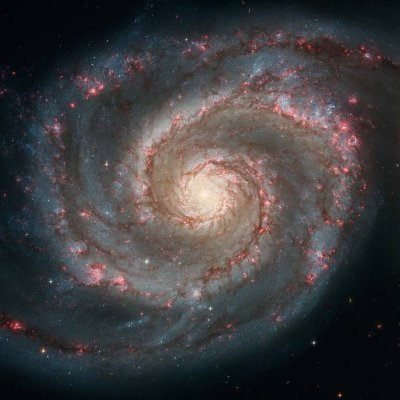
\includegraphics[width=5cm]{img/universe.jpg}
\end{figure}

Do you think the picture above is great?

\Blindtext[2]

AAAAAAAAAAAAAAAAAAAAAAAAAAAAAAAAAAAA

\blindtext

\section{Final part}

BBBBBBBBBBBBBBBBBBBBBBBBBBBBBBBB



\end{document}
